\documentclass[12pt,nofonts]{ctexart}
\usepackage{latexsym}
\usepackage{xeCJK}
\usepackage[noend]{algpseudocode}

\usepackage{algorithmicx,algorithm}
\setCJKmainfont[BoldFont=STFangsong]{STFangsong}
\setCJKmonofont{STFangsong}
\usepackage{geometry}
\geometry{a4paper,left=1.5cm,right=1.5cm,top=1.5cm,bottom=1.5cm}
\usepackage{amsmath}
\usepackage{amssymb}
\usepackage{cite}
\zihao{4}
\begin{document}

\title{生物智能算法课程报告-蚁群算法}
\author{王纪东 21621125}
\maketitle
\section{简介}
\subsection{背景}
人类认识事物的能力来源于与自然界的相互作用,自然界一直是人类创造力的源泉。自然界有许多自适应的优化现象不断地给人以启示,利用生物自身的演化能力解决了许多在人类看来高度复杂的优化问题。人类通过模拟自然生态系统来求解复杂优化问题的仿生学算法相继出现,如蚁群算法,遗传算法,粒子群算法等。

生物学家通过对蚂蚁的长期观察发现,每只蚂蚁的智能并不高,看起来没有集中的指挥,但它们却能协同工作,集中事物,建起坚固漂亮的蚁穴并抚养后代,依靠群体能力发挥出超出个体的智能。意大利学者Dorigo M\cite{ref0,ref4}等人在认真观察蚂蚁寻找食物的行为后,提出了蚁群算法,在研究了蚁群算法的基本原理和数学模型之后,结合了TSP优化问题与遗传算法,禁忌搜索算法,模拟退火算法等方法进行了仿真实验,为蚁群算法的发展奠定的了基础,并引起了全世界学者的关注与研究。
\subsection{蚂蚁寻路}
蚂蚁寻路本身是一个复杂的行为,原本难以用程序来计算,但是作者认为蚂蚁并不需要整个世界的信息,
他们只关心很小范围内的信息,而根据局部信息利用几条简单的规则进行决策,最终就能涌现出智能

1.范围
2.环境
3.觅食规则
4.移动规则
5.避障规则
6.播撒信息素规则

简单来说,蚂蚁在运动过程中会在经过的路径上留下一种信息素来传递信息,其他蚂蚁能够感知到这种物质,并以此知道自己的运动方向,因此由大量蚂蚁组成的蚁群集体行为便变现出一种信息正反馈的现象,某一路径上走过的蚂蚁越多,则后来选择该路径的概率就越大。
\begin{figure}
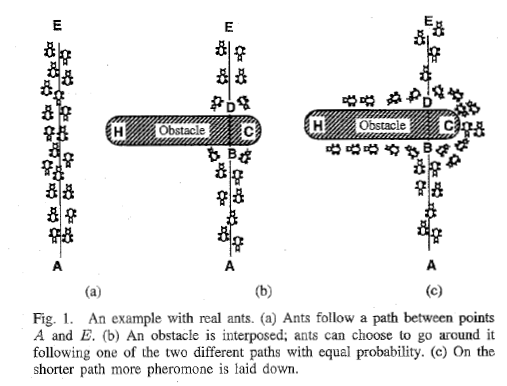
\includegraphics[width=\textwidth,height=0.4\textheight]{ants.png}
\end{figure}
\subsection{人工蚁群}
蚁群算法\cite{ref1}是从自然界中真实蚂蚁觅食的群体行为得到启发而提出的,其很多观点都来源于真实蚁群,因此算法中所定义的人工蚂蚁与真实蚂蚁存在如下共同点。
  (1)都存在一个群体中个体相互交流通信的机制
   人工蚂蚁和真实蚂蚁都存在一种改变当前所处环境的机制:真实蚂蚁在经过的路径上留下信息素,人工蚂蚁改变在其所经路径上存储的数字信息,该信息就是算
法中所定义的信息量,它记录了蚂蚁当前解和历史解的性能状态,而且可被其他后继人工蚂蚁读写。蚁群的这种交流方式改变了当前蚂蚁所经路径周围的环境,同
时也以函数的形式改变了整个蚁群所存储的历史信息。通常,在蚁群算法中有一个挥发机制,它像真实的信息量挥发一样随着时间的推移来改变路径上的信息量。
挥发机制使得人工蚂蚁和真实蚂蚁可以逐渐地忘却历史遗留信息,这样可使蚂蚁在选择路径时不局限于以前蚂蚁所存留的“经验”。
   (2)都要完成一个相同的任务
   人工蚂蚁和真实蚂蚁都要完成一个相同的任务,即寻找一条从源节点(巢穴)到目的节点(食物源)的最短路径。人工蚂蚁和真实蚂蚁都不具有跳跃性,只能在
相邻节点之间一步步移动,直至遍历完所有城市。为了能在多次寻路过程中找到最短路径,则应该记录当前的移动序列。
   (3)利用当前信息进行路径选择的随机选择策略
   人工蚂蚁和真实蚂蚁从某一节点到下一节点的移动都是利用概率选择策略实现的,概率选择策略只利用当前的信息去预测未来的情况,而不能利用未来的信息。
因此,人工蚂蚁和真实蚂蚁所使用的选择策略在时间和空间上都是局部的。
\section{蚁群算法}
\subsection{旅行商问题}
蚁群算法最早是用于解决旅行商问题,所以算法的定义也采用了旅行商的模型。旅行商问题(Traveling Salesman Problem,TSP)是旅行商要到若干个城市旅行,各城市之间的费用是已知的,为了节省费用,旅行商决定从所在城市出发,到每个城市旅行一次后返回初始城市,问他应选择什么样的路线才能使所走的总费用最短?此问题可描述如下:设$G=(V,E)$是一个具有边成本$d_{ij}$的有向图,$d_{ij}$的定义如下,对于所有的$i$和$j$,$d_{ij}>0$,若$<i,j>$不属于$E$,则$d_ij=∞$。令$|V|=n$,并假设$n>1$。 $G$的一条周游路线是包含$V$中每个结点的一个有向环,周游路线的成本是此路线上所有边的成本和。
\subsection{蚁群算法}
在蚁群优化算法(Ant Colony Optimization 简称ACO)\cite{ref2}中和自然蚁群一样,关键的因素就是信息素,它会影响蚂蚁的路径选择,最终保证算法收敛。参考自然蚁群,算法需要对蚂蚁经过的路径增加信息素,同时随着时间流逝,信息素会衰减。同时因为是群聚算法,所以肯定需要多个蚂蚁一起行动。由此我们可以得到蚁群算法的基本模型,
设$d_{ij}$为城市i,j之间的几何距离(欧式距离)。蚂蚁总数m,城市总数n,$\tau_{ij}$表示在t时刻在i,j
	连线上残留的信息量,初始时刻各条路径上的信息量为$\tau_{ij}=C_0$,用参数p表示信息量的保留度,则经过n个时刻后,路径ij上的信息量根据下试做调整

	$\tau_{ij}(t+n)=\rho \times \tau_{ij}(t)+\Delta\tau_{ij}$
	$\Delta\tau_{ij}=\sum_{k=1}^{m}\Delta\tau_{ij}^{k}$
	
	两个公式表达了信息素随着时间蒸发但是当蚂蚁走过时会增加。而$\Delta\tau_{ij}$表示第k只蚂蚁在本次循环中留在路径ij上的信息量为
	$\Delta\tau_{ij}^{k}=1/C^k$ ,如果边(i,j)在蚂蚁k的路径上。其中$C^k$为第k只蚂蚁所经历的路径总长度。
	同时定义$\eta_{ij}=\frac{1}{d_{ij}}$,表示蚂蚁看到的环境。则t时刻蚂蚁k由位置i转移到位置j的概率为

	$p_{ij}^{k}=\frac{\tau_{ij}^{\alpha}\eta_{ij}^{\beta}(t)}{\sum_{j\in allowed}\tau_{ij}^{\alpha}\eta_{ij}^{\beta}(t)}$
	由表达式可见蚂蚁转移的概率由信息素和当前城市间的距离共同决定

	同时我们也需要定义一个禁忌表记录蚂蚁已经走过的城市,目标城市在禁忌表中,则转移概率为0,防止蚂蚁再次访问,以保证每个城市都到达过一次。
\section{算法流程}
\begin{algorithm}[h]
\caption{蚁群算法} %算法的名字
\hspace*{0.02in} {\bf Input:} %算法的输入, \hspace*{0.02in}用来控制位置,同时利用 \\ 进行换行
城市距离矩阵 d,蚂蚁数量 m, C\\
\hspace*{0.02in} {\bf Output:} %算法的结果输出
最优路径
\begin{algorithmic}[1]
\State 初始化参数,信息路径之间信息量$\tau_{ij}=const$,其中const表示常数,初始时刻$\Delta\tau_{ij}=0$ % \State 后写一般语句
\While {没有收敛}
\For{t=1: n} % For 语句,需要和EndFor对应
	\For {k=1:m}
	\State 禁忌表索引号为k,蚂蚁k所在城市为i
	\For{j=1:n}
  \If{j不在禁忌表k中} % If 语句,需要和EndIf对应
    \State 计算转移概率$p_{ij}=\tau_{ij}^{\alpha}\eta_{ij}^{\beta}(t)$
  \Else
    \State 转移概率为0
  \EndIf
	\EndFor
	蚂蚁K根据概率$p_{ij}^{k}=\frac{\tau_{ij}^{\alpha}\eta_{ij}^{\beta}(t)}{\sum_{j\in allowed}\tau_{ij}^{\alpha}\eta_{ij}^{\beta}(t)}$选择下一个目的地,将蚂蚁移动到目的地城市,并且将目的地放入禁忌表中
	\EndFor
\EndFor
\State 统计所有蚂蚁的路径和,找出最短环路$C_k$,并更新所有路径上的信息素$\tau_{ij}(t+n)=\rho \times \tau_{ij}(t)+\Delta\tau_{ij}$,重置禁忌表
\EndWhile

\State \Return result
\end{algorithmic}
\end{algorithm}
1.当t=0时,将m个蚂蚁放在各城市,设定每条路径上的信息量初始值为C。

2.每个时刻t(t=1,2...n),蚂蚁k(k=1,2...m)根据公式计算的概率选择下一个要转移的城市。

3.经过n个时刻(总共有n个城市),所有的蚂蚁都完成了一次周游。计算每只蚂蚁所走过的路径长度,并保存最短的路径长度$L_{kmin}$,
同时按照公式更新路径上的信息素。%根据之前公示可知,蚂蚁经过的路径长度越小,则路径上各条边就会获得更多的信息素,信息素越多的边,在以后的迭代中就更有可能被其他蚂蚁选择。

4.蚂蚁完成一次周游后,重新回到初始城市,准备下一次周游。当周游次数达到设定值$N_{max}$或者所有蚂蚁选择相同路径时算法结束,输出最短路径为之前记录的最短路径中的最小值。
\section{优化分析}

蚂蚁每次走完所有城市,就在走过的路径留下信息素,后续的蚂蚁根据历史信息素的多少来选择要走的路径
如果蚂蚁的环游结果比较好,留下的信息素就比较多,从而使较好路径的被选择机会增加
经过多次循环,就可以逐渐凸现最好的路径。

实验表明,蚁群算法在解决小规模TSP问题时性能尚可,但是随着测试规模扩大(城市数大于50),算法性能同样下降的比较严重,很难在规定的循环次数中找出最优解来。
算法复杂度:O(最大循环数*蚂蚁数*城市数*城市数)
一个蚂蚁的需要在便利N个城市选择概率最大的一个,最终要选择N个城市。
而蚂蚁数一般选择和城市数一样。
所以算法的复杂度就是$O(T*N^3)$
而且在大规模TSP问题上ACO算法无法在有限时间内找到最优解,容易陷入局部最优局面,算法过早收敛。
\subsection{领域优化}
某些求解路径中会存在交叉路径,但存在交叉路径的情况下,结果一定不会是最好。所以配合领域优化算法进行优化,
\begin{figure}[h]
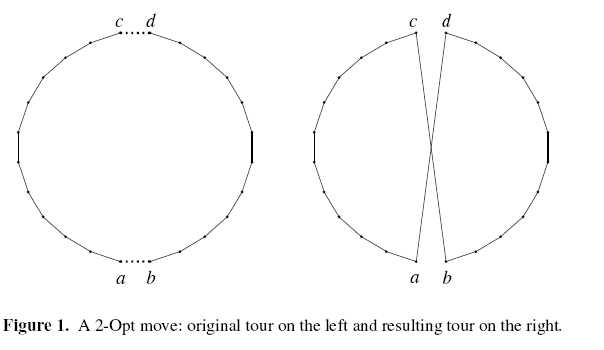
\includegraphics[width=\textwidth,height=0.4\textheight]{opt.png}
\end{figure}
算法的目的是做到:任意替换结果方案的两个路径,都不可能比结果方案更优,因此也就不可能存在交叉路径了,真是简单极了。

对于每一个蚂蚁产生的求解结果,都应用一次 2opt 邻域搜索
2opt 子过程不断地尝试所有的combin(n,2)个路径,如果替换这两个路径产生更好的结果,就保留结果并且重做整个2opt,直到仅仅交换两个路径根本无法产生更优结果为止。
\subsection{优化算法}
随着人们深入的研究,对蚁群算法做了许多改进,针对于信息量的更新方法,或者随机路径的选择等等,都对蚁群算法的优化效率有一定程度的影响
\begin{itemize}
		\item<1> 精英蚁群算法,跟基本蚁群算法几乎是完全一样的,只不过强调了“精英蚂蚁”的作用。
方法是:从所有已经走完环游的蚂蚁中,选择结果最好的蚂蚁,对其走过的路径,留下特别多的信息素
最好的蚂蚁可以选择A:从求解到现在最佳的蚂蚁,或者B:选择本次循环的最佳蚂蚁,效果其实差不多。
A方法的收敛速度快一点,B方法的随机性大一点,对很大规模很多次循环的求解,也许是B方法好一点。
这个增强版最大优点是实现非常简单,而且效果不错。

		\item<2> 最好最差蚁群 (BWAS)
这个算法几乎跟精英蚁群一样,也是保留一个精英蚂蚁,留下特别多的信息素。
但是增加了“最坏蚂蚁”的惩罚,本次循环的最差蚂蚁,其路径的信息素将多蒸发一次(如果这个路径也被最好蚂蚁走过,则不惩罚)
这个算法的性能只比精英蚁群好一点点。
		\item<3> 基于排名的蚁群(RAS)这个算法也跟精英蚂蚁一样原理:奖励比较好的蚂蚁。
不同的是,RAS除了奖励最佳蚂蚁,还奖励本次循环的多个蚂蚁,而且按多个蚂蚁的结果优劣,给与不同大小的奖励。
由于多个蚂蚁的随机性比一个蚂蚁强
所以这个算法的收敛性 低于 精英蚂蚁,也就是说,需要更多的循环数才能达到好结果。
但是求解结果比 精英蚂蚁要好一些,尤其是没有邻域搜索的情况下
		\item<4> 最大最小蚁群(MMAS)这个算法是目前性能最好的蚁群算法,发明者就是《Ant Colony Optimization》一书的第二作者 Thomas Stutzle
它的做法是:
1 跟之前所有蚁群算法不同,所有蚂蚁在走完环游之后,都不留信息素!
2 跟精英算法一样,选出最佳蚂蚁,最佳蚂蚁可以留信息素。
3 为了防止所有信息素都被蒸发掉,最后只剩下最佳蚂蚁的路径,MMAS采用很小的蒸发率,从而保证所有路径不会迅速变为0
4 强制所有路径的信息素,有最大值和最小值限制,高于低于这个范围都会被自动设置为最大值或者最小值
从而保证最少信息素的路径也有机会被选择
这个复杂的信息素规则,得到非常好的结果,即使不用邻域搜索,MMAS都可以直接求解出200以内规模的最优解!
非常强悍!
当然,由于蒸发率很低,所以要分出信息素的多和少(即路径的好与坏)
MMAS需要非常多的循环数,不用邻域搜索的话,推荐至少用3000循环。
		\item<5> 蚁群系统(ACS)1 它是唯一一个不带邻域搜索的时候,建议蚂蚁数为10的算法(其余各种增强版算法的建议蚂蚁数都是等于城市数)
所以不带邻域搜索的时候,它的速度是最快的,比其它算法低一个阶,快N倍吖!
2 它是唯一一个边走边改变信息素的算法,而且所有路径的信息素都不蒸发,如果没有蚂蚁走过,就一直不变!
ACS在每个蚂蚁走过某个路径时,该路径的信息素马上进行蒸发,而且所有蚂蚁都不留信息素!
也就是说,蚂蚁走过的路径,信息素不但不增加,而且还减少。
3 只有最佳蚂蚁留下信息素,也就是说最佳蚂蚁走过的路径,信息素才增加。
4 ACS连选择下一个城市的方法都不一样,ACS先固定一个“直接选择最多信息素路径”的概率Q
在每个蚂蚁选择城市的时候,先扔一个随机数,如果随机数低于Q,则直接选择“所有可选路径里面,信息素最多的那一个路径”(注:不一定是最接近的路径)
如果随机数大于Q,则采用基本蚁群算法的选择法,计算所有可选路径的信息素总和,计算每个路径的选择概率,再靠随机数决定选哪一个。
不过可惜的是,这么复杂的规则,其性能却并非最好,比不上MMAS。
另外,ACS的收敛速度虽然很高,但是却不稳定,也需要较多循环才能保证求解精度。
但非常值得一提的是,在没有邻域搜索的时候,ACS的速度是极快的。
现在,增强版的蚁群算法+邻域搜索,可以保证300以内的城市规模必定找到最优解(MMAS,多次循环+停滞检测+多次运行)
而1000以内的城市,求解精度一般不超过最优解的 103\%。

\end{itemize}
\subsection{缺点}
蚁群算法的研究成果令人瞩目,但作为一种较新的理论,它依然存在一些问题。

(1)对于大规模组合优化问题,算法的计算时间而且复杂。由于蚁群算法的时间复杂度是,因此在处理较大规模的组合优化问题时,运算量较大,时间较长。

(2)算法容易在某个或某些局部最优解的邻域附近发生停滞现象,造成早熟收敛,即搜索进行到一定程度后,所有蚂蚁发现的解完全一致,不能继续对解空间进一步搜索,不利于发现全局最优解。

(3)不能较好的解决连续域问题。

(4)由于蚁群算法中蚂蚁个体的运动过程的随机性,当群体规模设置较大时,很难在较短时间内从杂乱无章的路径中找出一条较好的路径。

(5)信息素更新策略,路径搜索策略和最优解保留策略都带有经验性,没有经过严格的理论论证。因此基本蚁群算法的求解效率不高、收敛性较差、求解结果具有较大的分散性。
\section{蚁群算法的应用}           
 蚁群算法最初被应用到经典的组合优化问题,随着研究的深入,应用范围扩大到更多的组合优化问题\cite{ref3},如在作业调度、网络路由、电力系统、生命科学、空战决策、聚类分析等领域都得到了广泛的应用,体现了蚁群算法的实用性和通用性。以下是几个蚁群算法应用的例子.
 \subsection{网络路由问题}
 将蚁群算法应用于解决受限路由问题,目前可以解决包括带宽、延时、丢包率和最小花费等约束条件在内的QoS组播路由问题,比现有的链路状态路由算法有明显的优越性。王卫亚等人将蚁群算法和遗传算法相结合的融合算法用于对带宽、时延和差率等多项QoS参数有要求的最优路由选择,在优化性能和时间性能上都取得了很好的效果。李俊等人提出了一种基于改进蚁群算法的分布式动态RWA方法,用于解决波分复用光网络中动态选路和波长分配问题,与现有最短路径相比,该算法有效降低了光路阻塞率,促进波长资源的合理分配,也降低了大型网络的通信开销。
 \subsection{电力系统领域}
 电力系统的许多优化问题本质上是属于组合优化问题。Gomez等人将蚁群算法应用于配电网络的规划。王林川等人将一种改进蚁群算法应用于配电网故障的定位。王海燕等人将蚁群算法应用于电力系统暂态稳定评估特征选择,减少了特征维数,提高了分类正确率。电力系统的这些组合优化问题的有效解决将为电力企业节省大量的资金,因此在电力系统的应用具有很大的实际价值。
 \subsection{飞行航迹规划}
 航迹规划是指在特定的约束条件下,寻找运动体从初始点到目标点满足某种性能指标最优的运动轨迹。在空防技术日益先进、防空体系日益完善的现代战争中,航迹规划是提高飞行器作战效能、实施远程精确打击的有效手段。因此对航迹规划方法的研究将有重要的现实意义。田伟等人提出了一种改进蚁群算法用于无人作战飞机的航路寻优过程,提高了无人作战飞机的航路寻优能力。孟祥恒等人将蚁群算法用于多无人机航迹规划。曹晋等人提出了一种基于蚁群算法的最小代价航迹规划方法,解决了航迹维数解算问题,为飞行器提供最优航迹规划路径。
\begin{thebibliography}{99}
 \bibitem{ref0}A. Colorni, M. Dorigo et V. Maniezzo, Distributed Optimization by Ant Colonies, actes de la première conférence européenne sur la vie artificielle, Paris, France, Elsevier Publishing, 134-142, 1991.
 \bibitem{ref4}M. Dorigo, Optimization, Learning and Natural Algorithms, PhD thesis, Politecnico di Milano, Italy, 1992.
\bibitem{ref1}吴庆洪, 张颖, 马宗民. 蚁群算法综述[J]. 微计算机信息, 2011, 27(3):1-2.
\bibitem{ref2}Xu B, Zhu J, Chen Q. Ant Colony Optimization[M]// New Advances in Machine Learning. InTech, 2010:1155-1173.
\bibitem{ref3}李士勇, 陈永强, 李研. 蚁群算法及其应用[M]. 哈尔滨工业大学出版社, 2004.
\end{thebibliography}
\end{document}